
% Copyright 2020 by Robert Hildebrand
%This work is licensed under a
%Creative Commons Attribution-ShareAlike 4.0 International License (CC BY-SA 4.0)
%See http://creativecommons.org/licenses/by-sa/4.0/
\chapter{Heuristics for TSP}
\todoChapter{ 50\% complete. Goal 80\% completion date: October 20\\
Notes: }

\todo[inline]{Add code from GUROBI webinar with models and heuristic examples and show plots of improvements}
\todo[inline]{Add links to resources from TSP video}
\todo[inline]{Create graphics using \url{https://www.manim.community/} and \url{https://github.com/nipunramk/Reducible}.}
In this section we will show how different heuristics can find good solutions to TSP.  For convenience,  we will focus on the \emph{symmetric TSP} problem.  That is, the distance $d_{ij}$ from node $i$ to node $j$ is the same as the distance $d_{ji}$ from node $j$ to node $i$.

There are two general types of heuristics: construction heuristics and improvement heuristics.  We will first discuss a few construction heuristics for TSP.


Then we will demonstrate three types of metaheuristics for improvement- Hill Climbing, Tabu Search, and Simulated Annealing.  These are called \emph{metaheuristics} because they are a general framework for a heuristic that can be applied to many different types of settings.  Furthermore, Tabu Search and Simulated Annealing have parameters that can be adjusted to try to find better solutions.  

\section{Construction Heuristics}
\subsection{Random Solution}
TSP is convenient in that choosing a random ordering of the nodes creates a feasible solution.  It may not be a very good one, but it is at least a solution.

\begin{general}{Random Construction}{Complexity: $O(n)$}
\label{heuristic:random}
For $i=1, \dots, n$, randomly choose a node not yet in the tour and place it at the end of the tour.
\end{general}

\subsection{Nearest Neighbor}
Starting from any node, add the edge to the next closest node.  Continue this process.
\begin{general}{Nearest Neighbor}{Complexity: $O(n^2)$}
\label{heuristic:nearestNeighbor}
\begin{enumerate}
\item Start from any node (lets call this node 1) and label this as your current node.
\item Pick the next current node as the one that is closest to the current node that has not yet been visited.
\item Repeat step 2 until all nodes are in the tour.
\end{enumerate}
\end{general}

\subsection{Insertion Method }
%\begin{general}{Insertion Method}{Complexity: $O(n^2)$}
%\label{heuristic:insertion}
%\begin{enumerate}
%\item Start from any 3 nodes (lets call this node 1) and label this as your current node.
%\item Pick the next current node as the one that is closest to the current node that has not yet been visited.
%\item Repeat step 2 until all nodes are in the tour.
%\end{enumerate}
%\end{general}
\begin{algorithm}
\caption{Insertion Method}
\label{heuristic:insertion}
\begin{algorithmic}[1]
    \State \textbf{Input:} Set of nodes, distance between nodes, etc.
    \State \textbf{Output:} Constructed tour.
    \State \textbf{Complexity:} $O(n^2)$

    \State Start from any 3 nodes (let's call the first one node 1) and label this as your current node.
    \While{there are unvisited nodes}
        \State Pick the next current node as the one closest to the current node that hasn't been visited yet.
    \EndWhile
    \State \Return the constructed tour.
\end{algorithmic}
\end{algorithm}

\section{Improvement Heuristics}
There are many ways to generate improving steps.  The key features of improving step to consider are
\begin{itemize}
\item What is the complexity of  computing this improving step?
\item How good this this improving step?
\end{itemize}

We will mention ways to find neighbors of a current solution for TSP.  If the neighbor has a better objective value, the moving to this neighbor will be an improving step. 


\subsection{2-Opt (Subtour Reversal)}
We will assume that all tours start and end with then node 1.  

\begin{general}{2-Opt (Subtour reversal)}{}
Input a tour $1 \to \dots \to 1$. 
\begin{enumerate}
\item Pick distinct nodes $i,j \neq 1$.
\item Let $s,t$ and $x_1, \dots, x_k$ be nodes in the tour such that it can be written as 
$$
1 \to \dots \to s \to i \to x_1 \to \dots \to x_k  \to j \to t \to \dots \to 1.
$$
\item Consider the subtour reversal
$$
1 \to \dots \to s \to j \to x_k \to \dots \to x_1  \to i \to t \to \dots \to 1.
$$
Thus, we reverse the order of $ i \to x_1 \to \dots \to x_k \to j$.  
\item In this process, we 
\begin{itemize}
\item deleted the edges $(s,i)$ and $(j,t)$
\item added the edges $(s,j)$ and $(i,t)$
\end{itemize}
\end{enumerate}
\end{general}
Pictorially, this looks like the following 

\refincludefigurestatic{wiki/File/2-opt_wiki.png}
%\begin{center}
%\includegraphics[scale = 0.25]{2-opt-1}
%\includegraphics[scale = 0.25]{2-opt-2}
%\includegraphics[scale = 0.25]{2-opt-3}
%\includegraphics[scale = 0.25]{2-opt-4}
%\includegraphics[scale = 0.25]{2-opt-5}\footnotemark
%\end{center}
%\footnotetext{Figures borrowed from unknown source.}

Computationally, we need to consider the costs on the edges of a graph.....


See 
\cite{Englert2014} for an analysis of performance of this improvement.
\subsection{3-Opt}


\subsection{$k$-Opt}
This is a generalization of 2-Opt and 3-Opt.

\section{Meta-Heuristics}

\subsection{Hill Climbing (2-Opt for TSP)}
The \emph{Hill Climbing} algorithm finds an improving neighboring solution and climbs in that direction.  It continues this process until there is no other neighbor that is improving.  

In the context of TSP, we will consider 2-Opt improving moves and the Hill Climbing algorithm for TSP in this case is referred to as the 2-Opt algorithm (also known as the Subtour Reversal Algorithm).
\begin{algorithm}
\caption{Hill Climbing}
\begin{algorithmic}[1]
    \State \textbf{Input:} Initial feasible solution, etc.
    \State \textbf{Output:} Best solution found.
    
    \State Start with an initial feasible solution, label it as the current solution.
    \Repeat
        \State List all neighbors of the current solution.
        \State Evaluate all neighbors to find the best one.
        \If{no neighbor is better}
            \State \textbf{break}
        \EndIf
        \State Move to the best neighbor.
    \Until{no better neighbor is found}
    \State \Return the current solution.
\end{algorithmic}
\end{algorithm}


Here is an example on the TSP problem with 2-Opt swaps:


\begin{longtable}{ccc}
\textbf{Current solution} & \textbf{Improvement Step} & \textbf{Reversal}\\
\hline
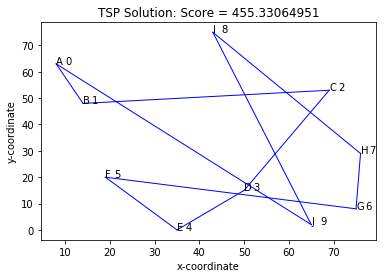
\includegraphics[scale = 0.4]{tsp-2-opt1} & 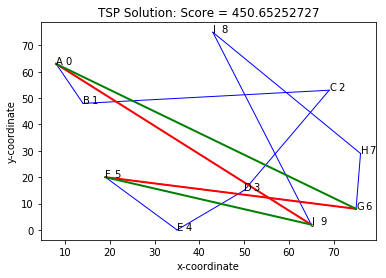
\includegraphics[scale = 0.4]{tsp-2-opt1-switch} & 
[A, B, C, D, E, F, \textbf{G, H, I, J}]
\\
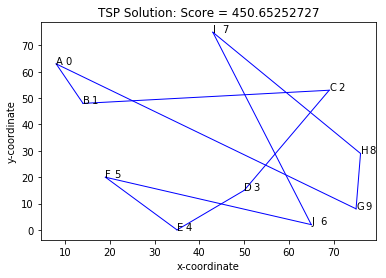
\includegraphics[scale = 0.4]{tsp-2-opt2} & 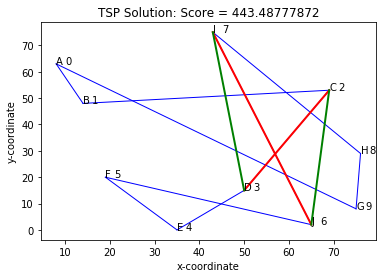
\includegraphics[scale = 0.4]{tsp-2-opt2-switch} & 
[A, B, C, \textbf{D, E, F, J}, I, H, G]\\
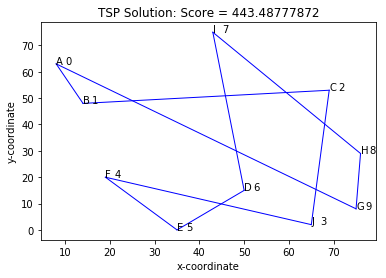
\includegraphics[scale = 0.4]{tsp-2-opt3} & 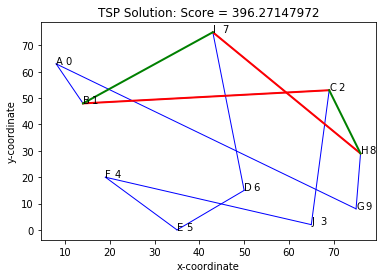
\includegraphics[scale = 0.4]{tsp-2-opt3-switch} & 
[A, B, \textbf{C, J, F, E, D, I}, H, G]
\\
%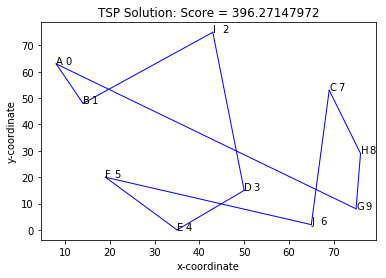
\includegraphics[scale = 0.4]{tsp-2-opt4} & 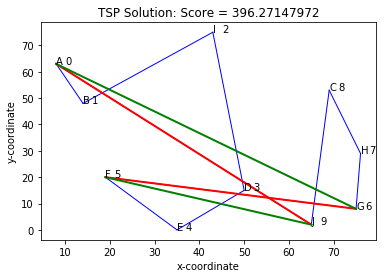
\includegraphics[scale = 0.4]{tsp-2-opt4-switch} & 
%[A, B, I, D, E, F, J, C, H, G]
%\\
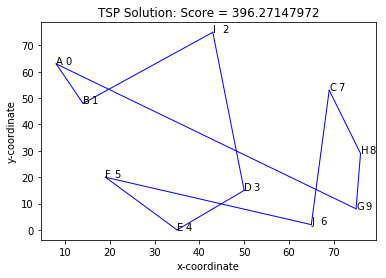
\includegraphics[scale = 0.4]{tsp-2-opt5} & 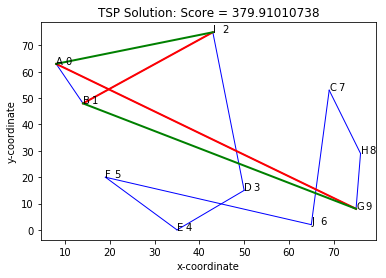
\includegraphics[scale = 0.4]{tsp-2-opt5-switch} & 
[A, B, \textbf{I, D, E, F, J, C, H, G}]
\\
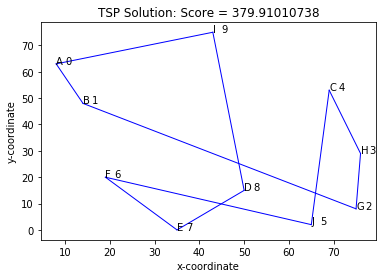
\includegraphics[scale = 0.4]{tsp-2-opt6} & 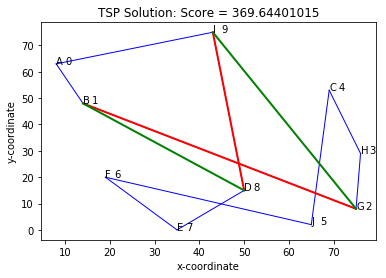
\includegraphics[scale = 0.4]{tsp-2-opt6-switch} & 
[A, B, \textbf{G, H, C, J, F, E, D}, I] 
\\
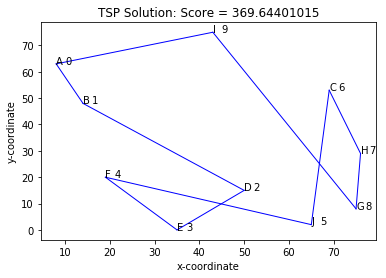
\includegraphics[scale = 0.4]{tsp-2-opt7} & 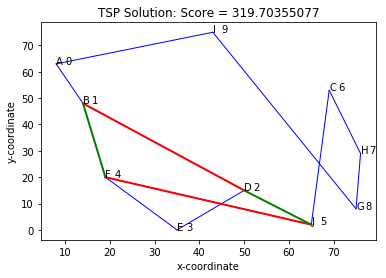
\includegraphics[scale = 0.4]{tsp-2-opt7-switch} & 
[A, B, \textbf{D, E, F}, J, C, H, G, I] 
\\
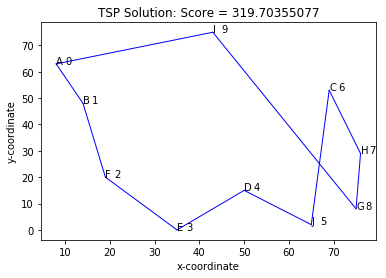
\includegraphics[scale = 0.4]{tsp-2-opt8} & 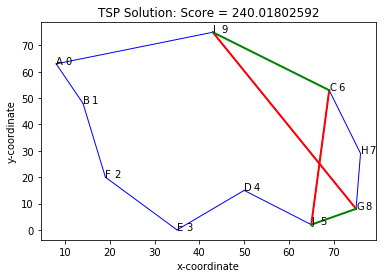
\includegraphics[scale = 0.4]{tsp-2-opt8-switch} & 
[A, B, F, E, D, J, \textbf{C,H,G}, I]  
\\
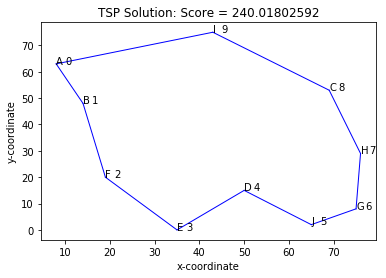
\includegraphics[scale = 0.4]{tsp-2-opt9} & No Improvement& 
[A, B, F, E, D, J, G, H, C, I] 
\\
\hline
\hline
\end{longtable}



\subsection{Simulated Annealing}

Here is a great python package for TSP Simulated annealing: \url{https://pypi.org/project/satsp/}.

Simulated annealing is a randomized heuristic that randomly decides when to accept non-improving moves.  For this, we use what is referred to as a \emph{temperature schedule}.  The temperature schedule guides a parameter $T$ that goes into deciding the probability of accepting a non-improving move.

A typically temperature schedule starts at a value $T = 0.2 \times Z_c$, where $Z_c$ is the objective value of an initial feasible solution.  Then the temperature is decreased over time to smaller values.

\textbf{Temperature schedule example:}
\begin{itemize}
\item  $T_1 = 0.2 Z_c$
\item $T_2 = 0.8 T_1$
\item $T_3 = 0.8 T_2$
\item $T_4 = 0.8 T_3$
\item $T_5 = 0.8 T_4$
\end{itemize}
For instance, we could choose to run the algorithm for 10 iterations at each temperature value.  The Simulated Annealing algorithm is the following:
\begin{algorithm}
\caption{Simulated Annealing Outline [minimization version]}
\begin{algorithmic}[1]
    \State \textbf{Input:} Initial feasible solution, temperature schedule, etc.
    \State \textbf{Output:} Best found solution during the algorithm.

    \State Start with an initial feasible solution, label it as the current solution, and compute its objective value $Z_c$.
    \While{iterations left in the schedule}
        \State Select a neighbor of the current solution and compute its objective value $Z_n$.
        \If{$Z_n < Z_c$}
            \State \textbf{accept the move} and set the neighbor as the current solution.
        \Else
            \State Compute $p = e^{\frac{Z_c - Z_n}{T}}$
            \State Generate a random number $x \in [0,1]$ from the computer.
            \If{$x < p$}
                \State \textbf{accept the move}
            \Else
                \State \textbf{reject the move} and stay at the current solution.
            \EndIf
        \EndIf
        \State Update the temperature $T$.
    \EndWhile
    \State \Return the best found solution.
\end{algorithmic}
\end{algorithm}


\refincludefigurestatic{simulated_annealing_temperatures.png}


\subsection{Tabu Search}
\todo[inline]{Connect to code example for general tabu search}
\begin{general}{Tabu Search Outline}{[minimization version]}
\begin{enumerate}
\item Initialize a \emph{Tabu List} as an empty set: $\textrm{Tabu} = \{ \}$.
\item Start with an initial feasible solution, label it as the current solution.
\item List all neighbors of the current solution.
\item Choose the best neighbor that is not tabu to move too (the move should not be restricted by the set $\textrm{Tabu}$.)
\item Add moves to the Tabu List.
\item If the Tabu List is longer than its designated maximal size $S$, then remove old moves in the list until it reaches the size $S$.
\item If no object improvement has been seen for $K$ steps, then Stop.
\item Otherwise, Go to Step 3 and continue.
\end{enumerate}
\end{general}


\subsection{Genetic Algorithms}
Genetic algorithms start with a set of possible solutions, and then slowly mutate them to better solutions.  See \href{https://github.com/guofei9987/scikit-opt}{Scikit-opt} for an implementation for the TSP.


\href{https://www.youtube.com/watch?v=XP8R0yzAbdo&ab_channel=FullstackAcademy}{Video explaining a genetic algorithm for TSP}

\subsection{Greedy randomized adaptive search procedure (GRASP)}
We currently do not cover this topic.  

\href{https://en.wikipedia.org/wiki/Greedy_randomized_adaptive_search_procedure}{Wikipedia - GRASP}

For an in depth (and recent) book, check out
\href{https://www.springer.com/gp/book/9781493965281}{Optimization by GRASP
Greedy Randomized Adaptive Search Procedures
Authors: Resende, Mauricio, Ribeiro, Celso C.}.

\subsection{Ant Colony Optimization}
\href{https://en.wikipedia.org/wiki/Ant_colony_optimization_algorithms}{Wikipedia - Ant Colony Optimization}

\section{Computational Comparisons}
Notice how the heuristics are generally faster and provide reasonable solutions, but the solvers provide the best solutions.  This is a trade off to consider when deciding how fast you need a solution and how good of a solution it is that you actually need.  


% Table for 5 nodes instance
\begin{table}[h]
\centering
\caption{Instance with 5 nodes}
\begin{tabularx}{\linewidth}{l c c c}
\toprule
Algorithm & Value & Time (seconds) & Memory \\
\midrule
Nearest Neighbor & 494 & 0.000065 & 2.172 KiB \\
Farthest Insertion & 494 & 0.000057 & 1.781 KiB \\
Simulated Annealing & 494 & 0.000600 & 162.156 KiB \\
Math Programming Cbc & 494.0 & 0.091290 & 1.460 MiB \\
Math Programming Gurobi & 494.0 & 0.006610 & 78.797 KiB \\
\bottomrule
\end{tabularx}
\end{table}

% Table for 20 nodes instance
\begin{table}[h]
\centering
\caption{Instance with 20 nodes}
\begin{tabularx}{\linewidth}{l c c c}
\toprule
Algorithm & Value & Time (seconds) & Memory \\
\midrule
Nearest Neighbor & 790 & 0.000162 & 6.406 KiB \\
Farthest Insertion & 791 & 0.000128 & 2.734 KiB \\
Simulated Annealing & 777 & 0.007818 & 2.601 MiB \\
Math Programming Cbc & 773.0 & 2.738521 & 607.961 KiB \\
Math Programming Gurobi & 773.0 & 0.238488 & 717.133 KiB \\
\bottomrule
\end{tabularx}
\end{table}

% Table for third instance (number of nodes not specified)
\begin{table}[h]
\centering
\caption{Instance with 40 nodes}
\begin{tabularx}{\linewidth}{l c c c}
\toprule
Algorithm & Value & Time (seconds) & Memory \\
\midrule
Nearest Neighbor & 1216 & 0.000288 & 15.141 KiB \\
Farthest Insertion & 1281 & 0.000286 & 3.969 KiB \\
Simulated Annealing & 1227 & 0.047512 & 10.387 MiB \\
Math Programming Cbc & 1088.0 & 6.292632 & 2.111 MiB \\
Math Programming Gurobi & 1088.0 & 1.349253 & 2.520 MiB \\
\bottomrule
\end{tabularx}
\end{table}

\subsection{VRP - Clark Wright Algorithm}
\todo[inline]{Include discussion of Clark Wright algorihtm, or link to earlier section on Algorithms}


\section*{Resources and References}
\begin{resource}

\begin{itemize}
\item \href{https://www.youtube.com/watch?v=GiDsjIBOVoA&ab_channel=Reducible}{Amazing video covering all TSP and topics in this section}
\item \href{https://cse442-17f.github.io/Traveling-Salesman-Algorithms/}{Interactive tutorial of TSP algorithms}
\item \href{https://www.youtube.com/watch?v=SC5CX8drAtU}{TSP Simulated Annealing Video with fun music.}
%\href{https://www.youtube.com/watch?v=SC5CX8drAtU}{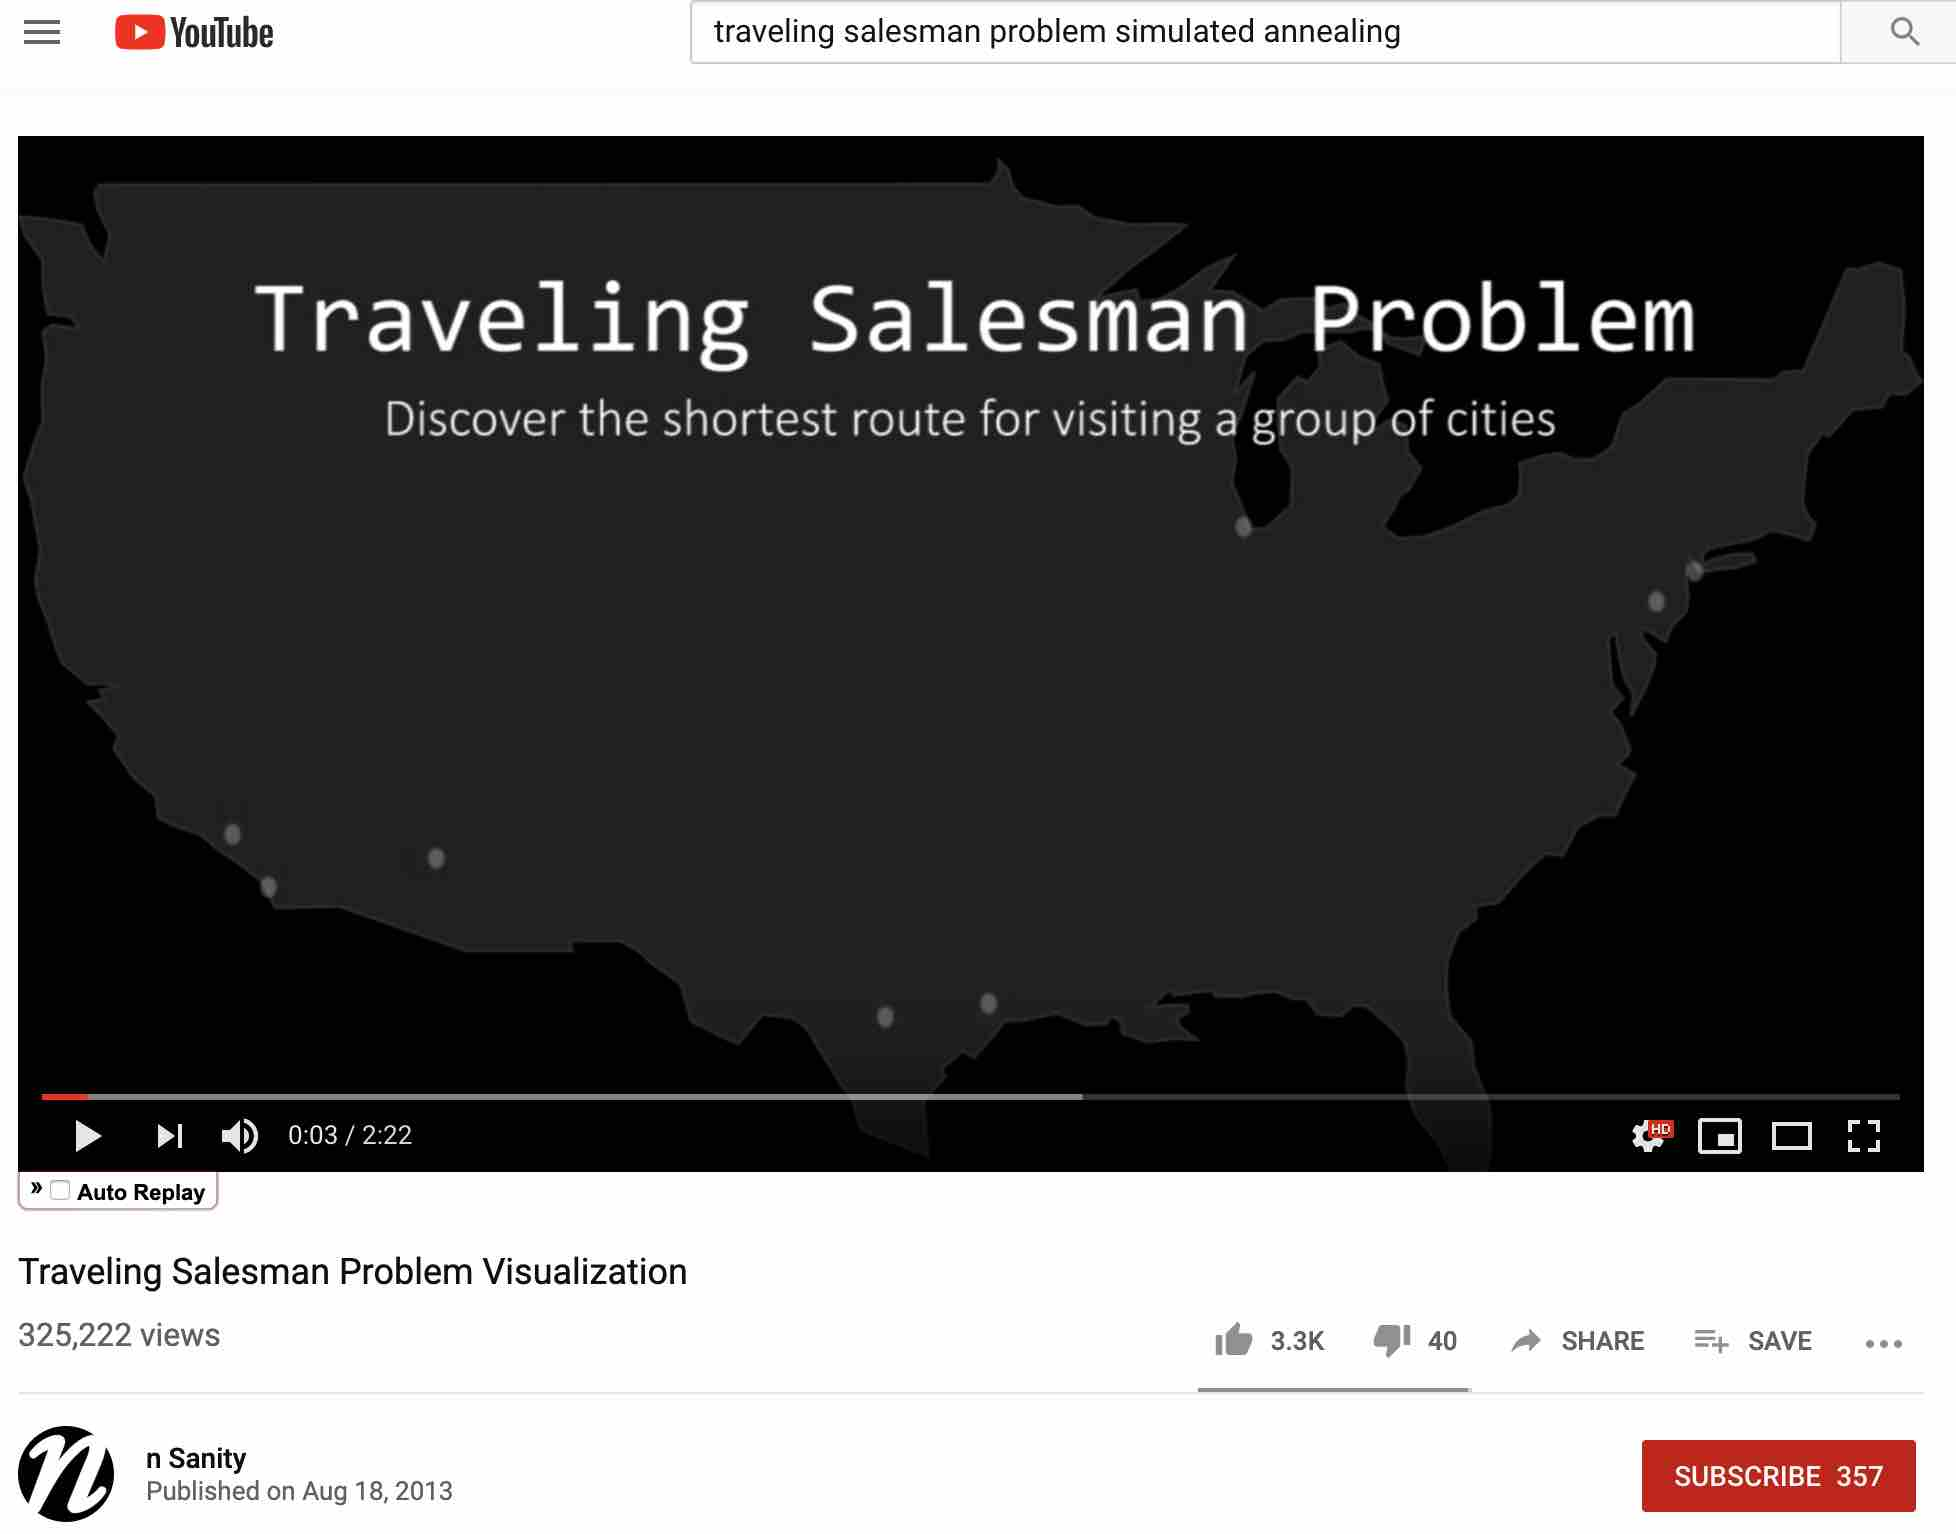
\includegraphics[scale = 0.13]{optimization/figures/figures-static/youtube-tsp-simulated-annealing}}
\item \href{https://www.youtube.com/watch?v=v9tUEsHD6BE&ab_channel=HasgeekTV}{VRP Heuristic Approach Lecture by Flipkart Delivery Hub}
\item \url{https://github.com/Gurobi/pres-mipheur} - Gurobi coded heuristics for TSP with comparison.  
\end{itemize}
\end{resource}

